%%%%%%%%%%%%%%%%%%%%%%%%%%%%%%%%%%%%%%%%%%%%%%%%%%%%%%%%%%%%%%%%%%%%%%%%%%%%%%%%%%%%%%%%%%%%%%%%%%%%%%%
%%%%%%%%%%%%%% Template de Artigo Adaptado para Trabalho de Diplomação do ICEI %%%%%%%%%%%%%%%%%%%%%%%%
%% codificação UTF-8 - Abntex - Latex -  							     %%
%% Autor:    Fábio Leandro Rodrigues Cordeiro  (fabioleandro@pucminas.br)                            %% 
%% Co-autor: Prof. João Paulo Domingos Silva  e Harison da Silva                                     %%
%% Revisores normas NBR (Padrão PUC Minas): Helenice Rego Cunha e Prof. Theldo Cruz                  %%
%% Versão: 1.0     13 de março 2014                                                                  %%
%%%%%%%%%%%%%%%%%%%%%%%%%%%%%%%%%%%%%%%%%%%%%%%%%%%%%%%%%%%%%%%%%%%%%%%%%%%%%%%%%%%%%%%%%%%%%%%%%%%%%%%
\section{\esp Introdução}

Instituída em 10 de dezembro de 2009, a Lei n.º 12.116/2009 \citeonline{lei12116}, conforme o Congresso Nacional Brasileiro, decreta o dia 27 de novembro como o Dia Nacional de Luta contra o Câncer de Mama. Além de uma data específica para a luta contra esse câncer, foi criada, em 1990, uma campanha cujo objetivo é conscientizar a população sobre a importância da prevenção e do diagnóstico precoce, o chamado Outubro Rosa.

Causado pela multiplicação rápida e desordenada de células anormais, o câncer pode ocorrer em diversas estruturas do corpo, e quando envolve as células das glândulas mamárias, determina o câncer de mama \cite{incaoquee}. Esse tumor divide a primeira posição com o de pulmão no ranking dos cânceres mais incidentes do mundo, além de ser a doença mais comum entre as mulheres, na qual dados da Organização Mundial de Saúde (OMS) e do Instituto Nacional de Câncer (INCA) apontam que houve por volta de 627 mil mortes por câncer de mama no mundo em 2018, sendo 17,7 mil no Brasil \cite{boletimepidemiologico}.

O diagnóstico prévio dessa doença tem alta significância na contenção do progresso da doença, devido à introdução antecipada do tratamento, que favorece o crescimento das chances de sobrevivência do paciente diagnosticado. Diante disso, existem alguns procedimentos basilares empregados para o diagnóstico dessa doença, tais quais: o exame de toque; exames clínicos; exames de imagens como a mamografia, ultrassonografia ou ressonância magnética; e a confirmação via biópsia.

% \subsection{\esp Problema Escolhido}
% Já está incluso nesse parágrafo (sobre imagens termográficas)
De acordo com \citeonline{borchartt}, a mamografia é o exame mais comum para a detecção do câncer de mama, mas apresenta algumas limitações, especialmente para mulheres mais jovens e com o tecido mamário denso. Perante o avanço computacional, a termografia se destaca como uma técnica de diagnóstico não invasiva que permite interceptar diferenças de temperatura em diferentes regiões do corpo através da intensidade da radiação infravermelha. Quando aplicada ao câncer de mama, a termografia se torna uma ferramenta essencial para a detecção precoce da doença. Isso porque as células cancerígenas tendem a apresentar temperaturas mais elevadas do que as células normais, independentemente de fatores como idade e outros \cite{leles}.

% \subsection{\esp Motivações}
Com a evolução da computação em diversos âmbitos tecnológicos, tais como redes neurais, processamento de imagens e inteligências artificiais, oportunidades foram criadas para investigar e implementar soluções avançadas na área da saúde, visando agregar a comunidade médica, além da sociedade no geral. Na oncologia, existem diversos métodos e práticas utilizadas para diagnosticar um quadro de câncer de um paciente, porém, em sua grande maioria, requer uma análise humana que é passiva de erros ou até mesmo incapaz de realizar predições, ou quantificar com precisão o diagnóstico do quadro clínico.

Pautando-se na ideia de trazer ferramentas, compostas por algoritmos avançados que auxiliam médicos no diagnóstico precoce do câncer de mama, assim melhorando na tomada de decisões dos profissionais de saúde acerca do quadro geral dos pacientes, iniciando tratamento previamente, garantindo uma qualidade de vida e uma longevidade maior para todos assolados pelo quadro de câncer.

% \subsection{\esp Objetivos}
Por meio dos tópicos apresentados, o presente artigo aspira discorrer sobre uma metodologia para o estudo de imagens termográficas, identificando as células como cancerosas utilizando aprendizado por transferência. Outrossim, para investigar de maneira experimental o tema proposto neste artigo, serão empregadas bases de dados, criteriosamente selecionadas e normalizadas em termos de tamanho e histograma, contendo amostras de mamografias para o treinamento de um programa de inteligência artificial a ser desenvolvido. As amostras serão divididas em mamografias sem sinais de câncer, e mamografias com câncer, classificadas de acordo com seus respectivos graus.

%(Não entra na introdução. Não é necessário) - Tava entre "transferência. (AQUI). Outrossim, para ". De maneira mais intrínseca, serão feitas análises de trabalhos correlatos a fim de alargar os conhecimentos no tema escolhido e contextualizar o leitor, além da exploração de artigos com o intuito de poder referenciá-los no presente artigo, ocasionando veracidade, autenticidade e acurácia para o artigo.

Para criar um modelo de classificação de graus, será utilizado o método de \textit{Deep Learning}, que consiste em uma técnica avançada de aprendizado de máquina. Após o treinamento do modelo, sua acurácia será avaliada por meio de testes, e assim que devidamente treinado, o programa será capaz de analisar as imagens dos exames mamográficos e realizar uma classificação precisa e automatizada do câncer de mama, identificando o grau da doença, caso presente no paciente.







\section{Fundamentação teórica} 
%10 artigos
%Usado 1 artigo: Souza (2018)
A fim de fornecer informações mais detalhadas sobre os tópicos vitais para a compreensão do presente artigo, serão retratados conceitos fundamentais sobre o câncer de mama, exames e tratamentos para a doença, bem como técnicas de processamento de imagens termográficas. Além disso, será discutida a técnica de \textit{Transfer Learning} com o uso de imagens para demonstrar sua relevância no contexto da detecção do câncer de mama.

\subsection{Câncer de mama}
As células vivas que compõem o corpo humano se dividem para permitir o crescimento e a substituição de células danificadas ou mortas. A proliferação celular é regulada pelos genes do DNA, transmitidos pelos pais e gerenciados para manter o equilíbrio no processo de divisão celular. O câncer, em geral, se forma quando esse controle genético é danificado ou perdido em uma, ou mais células que então continuam a se dividir normalmente, produzindo mais células anormais, causando danos a outros tecidos e funções corporais \cite{basicOncology}.

O câncer de mama, em específico, se dá pelo crescimento de células anormais na glândula mamária, e os sub-tipos diferentes desse câncer estão localizados sob o tecido adiposo\footnote{tecido que armazena gordura e mantém a maior reserva de energia do organismo} e no sistema ductal\footnote{ductos responsáveis por conduzir o leite até a papila}. Conforme apontado por \citeonline{souza}, o câncer de mama apresenta células com uma taxa de duplicação de tamanho estimada em 4 meses. Embora o crescimento seja inicialmente lento, quando o tumor se torna palpável e não é tratado, o câncer pode se disseminar para os linfonodos, pulmões, ossos, fígado e cérebro, desenvolvendo metástase.

%3o paragrafo: falar um pouco sobre exames (mamografia e por que não é tão confiável quanto imagens termograficas) - pegar outro artigo



\subsection{Técnicas de processamento de imagem}
%3 paragrafos
A definição básica de processamento de imagem refere-se ao processamento da imagem digital, ou seja, remover o ruído e qualquer tipo de irregularidades presentes em uma imagem usando o computador digital. O ruído ou irregularidade pode se infiltrar na imagem durante sua formação ou durante a transformação, etc. Para análise matemática, uma imagem pode ser definida como uma função bidimensional f(x, y) onde x e y são coordenadas espaciais (planas) e a amplitude de f em qualquer par de coordenadas (x, y) é chamada de intensidade ou nível de cinza da imagem naquele ponto. Quando x, y e os valores de intensidade de f são todas quantidades finitas e discretas, chamamos a imagem de imagem digital. É muito importante que uma imagem digital seja composta de um número finito de elementos, cada um com uma localização e valor específicos. Esses elementos são chamados de imagem elementos, elementos de imagem, pels e \textit{pixels}. \textit{Pixel} é o termo mais amplamente usado para denotar os elementos de uma imagem digital.

Colocar imagem aqui.

Várias técnicas foram desenvolvidas em processamento de imagem durante as últimas quatro a cinco décadas. A maioria dos técnicas são desenvolvidas para aprimorar imagens obtidas de espaçonaves não tripuladas, sondas espaciais e militares de voos de reconhecimento. Os sistemas de processamento de imagem estão se tornando populares devido à fácil disponibilidade de pessoal poderoso computadores, dispositivos de memória de grande porte, software gráfico, etc. A principal vantagem dos métodos de processamento de imagem digital é a sua versatilidade, repetibilidade e preservação da precisão dos dados originais. As várias técnicas de processamento de imagem são:

\begin{enumerate}
        \item Pré-processamento de imagem
        \item Melhoria de imagem
        \item Segmentação de imagem
        \item Extração de recursos
        \item Classificação de imagem
\end{enumerate}

\newpage

Às vezes, imagens obtidas de satélites e câmeras convencionais ou digitais carecem de contraste e brilho devido às limitações dos subsistemas de imagem e condições de iluminação durante a captura da imagem. As imagens podem ter diferentes tipos de ruído. No aprimoramento de imagem, o objetivo é acentuar certas características da imagem para análise posterior ou para exibição de imagens. Os exemplos incluem contraste e aprimoramento de borda, pseudo-coloração, filtragem de ruído, nitidez e ampliação. O aprimoramento de imagem é útil na extração de recursos, análise de imagem e exibição de imagem. O próprio processo de aprimoramento não aumenta o conteúdo de informações inerentes aos dados. Ele simplesmente enfatiza certas características de imagem especificadas. Algoritmos de aprimoramento são geralmente interativos e dependentes de aplicativos. Algumas das técnicas de aprimoramento são:

\begin{enumerate}
        \item Alongamento de contraste
        \item Filtragem de Ruído
        \item Modificação do histograma
\end{enumerate}


\subsection{Transfer Learning}
%3 paragrafos
%O que a gnt vai usar é transfer learning. Explicar um pouco sobre transfer learning (que é um método de machine learning) e ver a aplicação dele dentro do deep learning.
%Qual approach?
%   Develop Model Approach
%   Pre-trained Model Approach
%Uma aplicacao de transfer learning com deep learning é o transfer learning com image data.
%It is common to perform transfer learning with predictive modeling problems that use image data as input.






\section{\esp Trabalhos correlatos} %10 artigos
%Usado 1 artigo: Rajinikanth (2021)
%   Trabalhos com o tema PARECIDO. 
%       Qual o problema que o artigo correlato resolve (cancer de mama, outra doenca)? 
%       Qual o contexto? 
%       O que eles estão propondo? 
%       Estão usando quais técnicas/metodos? 
%       O quão bom foram os resultados que eles tiveram (assertividade ou outras métricas)? 
%

Neste tópico, serão abordados trabalhos correlatos ao diagnóstico de câncer utilizando inteligência artificial, porém se diferenciado em termos médicos, como o diagnóstico de outras doenças, em termos de tipo de entrada a ser computada, como radiografias, ou até mesmo imagens digitais. As análises dos trabalhos relacionados também se diferenciarão em termos de abordagem, utilizando-se de outros algoritmos de \textit{Machine Learning}. Além disso, serão feitas analises das propostas dos trabalhos, além dos resultados e assertividades.


Em \citeonline{marinePredators}, a avaliação de desempenho das diferentes classificações são executadas e baseadas na classificação de acurácia. Foi proposto chegar em uma acurácia maior ou igual à 92\% para o diagnóstico de câncer de mama utilizando imagens termográficas, normalizando-as e utilizando duas abordagens de extração de recursos: (i) o método \textit{Grey Level Co-Occurence Matrix} (GLCM) e (ii) o método \textit{Local Binary Patterns} (LBP). O GLCM é uma matriz que representa a distância e a relação espacial angular sobre uma sub-região de imagem de uma região específica. Além disso, ela ajuda a pegar informações sobre forma e textura da imagem. Já o LBP consegue extrair características estruturais de uma imagem por meio de histogramas locais, baseados na vizinhança dos \textit{pixels} vizinhos.

%Giovanna em 2023-04-26: Outro artigo \citeonline{comparing} - A acurácia é somente de 61,7%. Falar sobre o que foi feito.

%Giovanna em 2023-04-26: \citeonline{botelho} não é sobre cancer de mama, é cancer de pele. usa redes neurais





\subsection{Outros métodos de aprendizado de máquina}
falar sobre o marine-predators-algorithm
\subsection{Outros tipos de imagens a serem processadas?}
\subsection{Outros tipos de canceres e diferenças entre análise de imagens?}

% \section{\esp Desenvolvimento}

% Todo título de seção ou subseção deverá ser seguido de texto.
% Para as seções textuais utilizar numeração progressiva em algarismos arábicos, limitada até a seção quinária 
% (NBR 6024/2003) da ABNT. Devem ser diferenciadas utilizando os recursos gráficos abaixo \cite{manualpuc}.
% Os títulos das seções primárias devem ser em caixa alta, negrito, tamanho 12.

% \subsection{\esp Seção secundária}

% Os títulos das seções secundárias terão caixa baixa, negrito, tamanho 12.

% \subsubsection{\esp Seção terciária}

% Caixa baixa, itálico, negrito, tamanho 12.

% \subsubsubsection{\esp Seção quartenária}
 
%  Caixa baixa, sublinhado, negrito, tamanho 12.
 
%  \subsubsubsubsection{\esp Seção quinária}
 
%  Nas seções quinárias, deve ser usado caixa baixa, sem negrito, tamanho 12.

% \section{\esp Elementos flutuantes}

% Elementos inseridos no texto como imagens, tabelas, algoritmos etc.
% Recomenda-se a colocação das ilustrações de forma centralizada, dentro das margens. 
% Caso não seja possível, em \citeonline{manualpuc} recomenda-se utilizar recursos como: 
%  a) utilizar letras com tamanho menor ao padrão do texto; a) imprimir a ilustração no sentido vertical; 
%  c) imprimir em folha A3 ou superior e dobrá-la até atingir o tamanho da folha A4. 

% Nas normas da PUC é afirmado a necessidade de se observar que todos os elementos flutuantes inseridos devem ter a formatação básica:

% \begin{enumerate} 
%  \item [a)] Título centralizado localizado na parte superior; 
%  \item [a)] Fonte em tamanho 10 na parte inferior;
%  \item [c)] Devem ser inseridas o mais próximos do texto que as referenciam.
% \end{enumerate}


% \subsection{\esp Inserções de ilustrações}

% As ilustrações devem ser inseridas seguindo o exemplo da Figura \ref{fig:figura1}. 
% % Figura
% \begin{figure}[ht]
% 	\centering	
% 	\caption[\hspace{0.1cm}Grade Computacional.]{Uma Grade Computacional como fonte transparente}
% 	\vspace{-0.4cm}
% 	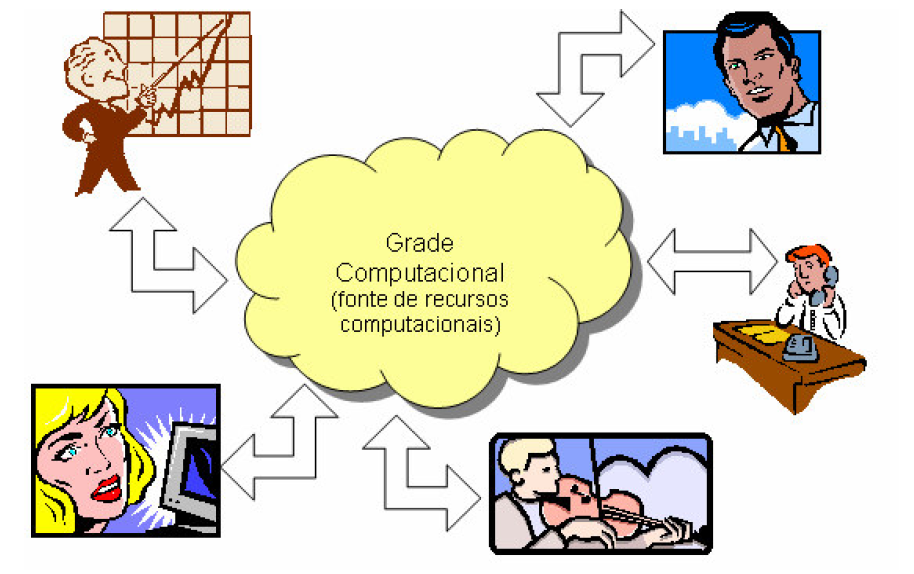
\includegraphics[width=0.6\textwidth]{figuras/grade-comp.png}
% 	% Caption centralizada
% % 	\captionsetup{justification=centering}
% 	% Caption e fonte 
% 	 \vspace{-0.2cm}
% 	\\\textbf{\footnotesize Fonte: \cite{cap-livro} }
% 	\label{fig:figura1}
% \end{figure}
% \vspace{-0.5cm}

% \subsection{\esp Inserção de tela de software}

% Nos casos de telas de \textit{software}, devem ser inseridas como figuras, e referenciadas no texto
% como na Figura \ref{fig:tela1}. Além disso, é necessário que seja citada no texto a empresa desenvolvedora.

% % Figura
% \begin{figure}[!ht]
% 	\centering	
% 	\caption[\hspace{0.1cm}Exemplo de tela de software.]{Exemplo de tela de software}
% 	  \vspace{-0.4cm}
% 	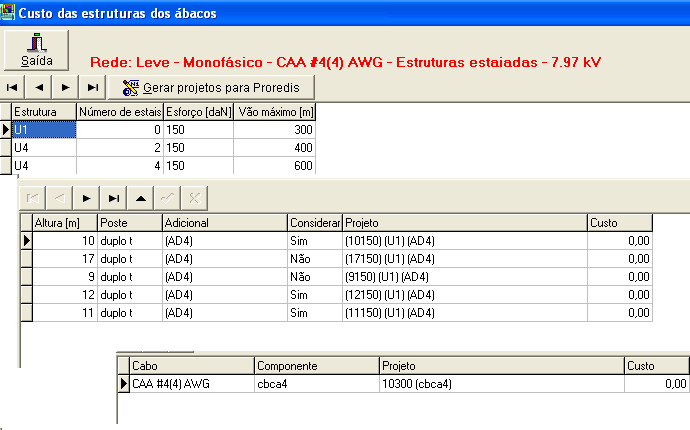
\includegraphics[width=.8\textwidth]{figuras/tela1.png}
% 	% Caption centralizada
% % 	\captionsetup{justification=centering}
% 	% Caption e fonte
% 	 \vspace{-0.3cm}
% 	\\\textbf{\footnotesize Fonte: \cite{tela1}}
% 	\label{fig:tela1}
% \end{figure}

% \subsection{\esp Inserção de gráficos e mapas}

% O gráfico é um tipo de ilustração que deve conter todos os elementos citados e também a descrição de seu título
% diferenciando-o das figuras da mesma forma que no Gráfico 1. 

% \begin{center}
% 	\centering	
%  	\textbf{Gráfico 1 - Exemplo de um gráfico} \\
% %  	  \vspace{0.cm}
% 	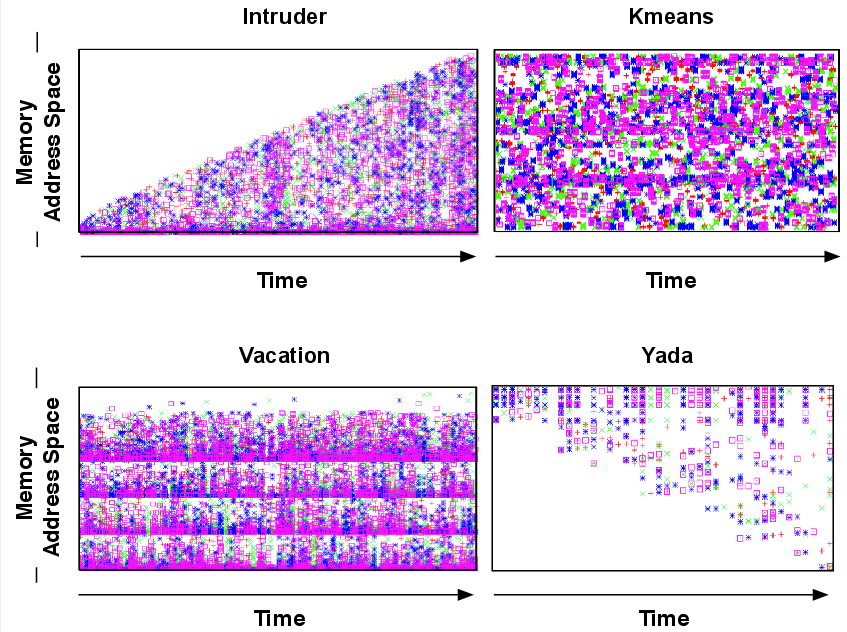
\includegraphics[width=0.7\textwidth]{figuras/access.png}
% 	% Caption centralizada
% % 	\captionsetup{justification=centering}
% 	% Caption e fonte
% 	 \vspace{-0.3cm}
% 	\\\textbf{\footnotesize Fonte: \cite{tese}}
% 	\label{grafico1}
% \end{center}

% A mesma regra se aplica para mapas, que devem ser adicionados seguindo as regras de apresentação já mostradas. No caso específico,
% o título e a numeração, também como os gráficos, devem começar do numeral ``1'' depois da marcação ``Mapa'' seguido do nome do elemento.
% Exemplo: \textbf{Mapa 1 - Exemplo de um Mapa}.

%  \subsection{\esp Tabelas}

% As tabelas devem ser abertas nas laterais, com espaços verticais separando
% as colunas e sem espaços horizontais, exceto na
% separação do cabeçalho. Um exemplo é a Tabela \ref{tab:tabela1}. 

% % Tabela
% \begin{table}[htb]
% 	\centering
% 	\caption{\hspace{0.1cm} Exemplo de uma tabela}
% 	\vspace{-0.3cm} % espaço entre titulo e tabela
% 	\label{tab:tabela1}
% 	% Conteúdo da tabela
% 	\begin{tabular}{l|c|c}
%   \hline
%     \textbf{Imagem}	& \textbf{transferência} & \textbf{tempo} \\
%     \hline
%      estação 1	& 7,72 MB/s &  1:22:18 \\
%      estação 2	& 7,72 MB/s &  1:22:17 \\
%      estação 3	& 7,59 MB/s & 1:24:25 \\
%      estação 4  & 7,53 MB/s & 1:43:27 \\
%      estação 5	& 6,14 MB/s  &  1:24:41 \\
%      estação 6  &  7,50 MB/s & 1:23:53 \\
%      estação 7  & 7,58 MB/s  &  1:24:02 \\
%      estação 8  & 7,8 MB/s  &  1:29:06 \\
%      estação 9  & 7,9 MB/s  &  1:30:05 \\
%      estação 10 & 8,0 MB/s  &  1:32:03 \\
%      \hline
%  \end{tabular}
%  	\vspace{.1cm}  %espaço entre tabela e fonte
% 	\small
% 	% Fonte
% 	{\footnotesize\\ \textbf{Fonte: \cite{monog-fabio}}}
% \end{table}

% \subsection{\esp Quadros}

% Os quadros diferem das tabelas por apresentarem dados textuais.
% Esses dados podem ser esquemáticos, comparativos ou descritivos.

%    \begin{center}
%           \centering
%        	\textbf{Quadro 1 - Bandas/Artistas de Rock e outros}\\
% % 	\vspace{-0.3cm} % espaço entre titulo e tabela
%         \label{quadro1}
% 	\begin{tabular}{|c|c|c|c|} \hline
% 	\multicolumn{4}{|c|}{\textbf{Bandas ou Artigas de Rock e outros}} 	  \\ 
% 		\hline \textbf{	Progressivo} & Pink Floyd & Jethro Tull	& Yesterday \\ 
% 		 \hline \textbf{ Metal}  & Metallica & Iron Maidam & Black Sabath \\ 
% 		\hline \textbf{	Arena Rock} & Led Zeppelin & The Rolling Stones & Beatles \\ 
% 		\hline \textbf{ Punk} & Ramones & Black Flag & NOFX	\\ 
% 		\hline \textbf{	Nacional} & Ira & Engenheiros & Vinil	\\ 
% 		\hline \textbf{	S.J.E.} & Apolo XI & Invasão 7 & Por do Sol \\ 
% 		\hline \textbf{	Grunge} & Nirvana & Pear Jam & Alice in Chains	\\ 
% 		\hline \textbf{	Rock Folk} & Bod Dylan & The Byrds &  The Mamas \& the Papas \\
% 		\hline \textbf{	Blues} & B.B. King & Albert Colins & Mady Wathers \\ 
% 		\hline \textbf{	New Wave} & The Police & The Pretenders, &  Duran Duran\\ 
%  		\hline \textbf{	Rock Folk} & Bod Dylan & The Byrds &  The Mamas \& the Papas \\
%  		\hline \textbf{	Rock alternativo} & R.E.M.& Hüsker Dü & Big Black\\ 
 		
% 		\hline
% 	\end{tabular}
% 	\vspace{0.1cm} 
% 	{\footnotesize\\ \textbf{Fonte: Dados da pesquisa}}
%    \end{center}

% Para gráficos, quadros e tabelas, cujos dados foram extraídos da própria pesquisa, 
%  usar a expressão: Dados da pesquisa. Ver exemplo no Quadro 1.
   

% \subsection{\esp Inserção de algoritmos}

% Para inserir um algoritmo, utilizar o exemplo do Algoritmo  \ref{alg:rnagenerica}.
% Todos os algoritmos devem ser inseridos como figura, indicada por nome e  fonte. Caso 
% forem de própria autoria, isso deverá ser mencionado na fonte, como elaboração feita pelos autores.

% % algoritmo
% % \begin{figure}[ht]
% \begin{center}	
% 	% Arquivo da figura
% % 	\caption[\hspace{0.1cm} Texto da figuras.]{Algorítmo CAC RD Neural}
%          \textbf{Algoritmo 1 -  CAC RD Neural}
% 	\vspace{-0.3cm}
% \begin{minipage}[ht]{13cm}
% \begin{algorithm}[H]
%   \footnotesize
%   \caption{CAC-RD Neural}
%   \label{alg:rnagenerica}
%   \begin{algorithmic}[1]
%       \STATE \textbf{Entrada:} Requisição da chamada
%     \STATE \textbf{Saída:} Aceitação ou bloqueio da solicitação
    
%     \STATE Preenche o vetor de $attributes.size+1$ atributos com os valores dos atributos, sendo a primeira posição do vetor preenchida com o valor 1
% 		\STATE $hidden\_layer\_size =  attributes.size*2+1;$

%     \FOR{$i$ = 1 to $attributes.size+1$}
%     	\STATE \textbf{normalizar}($Entrada_i$)
%     \ENDFOR

% 		\STATE $double [] net = new double [hidden\_layer\_size];$
%     \STATE $net = hidden\_layer\_weights * attributes;$
%    	\FOR{$i$ = 0 to hidden\_layer\_size}
% 			\STATE $net [i] = 1.0 / (1.0 + exp((-1.0)*net[i]));$
% 		\ENDFOR

% 		\STATE $double [] ipVector = new double [hidden\_layer\_size+1];$
%     \STATE $ipVector [0] = 1.0;$
%    	\FOR{$i$ = 1 to $hidden\_layer\_size+1$}
% 			\STATE $ipVector [i] = net [i-1];$
% 		\ENDFOR
		
% 		\STATE $output = output\_layer\_weights *  ipVector;$
%     \STATE output = \textbf{desnormalizar}(Saída)
%     \STATE \textbf{net\_update} (requisition);
    
%     \STATE \textbf{Retorna} output; FIM
%   \end{algorithmic}
% \end{algorithm}
% % \vspace{-0.3cm} % espaço entre algoritmo e fonte

% \small \centering \textbf{\footnotesize Fonte: \cite{mestrado}.}
% \end{minipage}
% \end{center}
% % \end{figure}

% Para ilustrações criadas ou adaptadas a partir de outras ilustrações, usar as expressões: 
% “Adaptado de...” ou “Criado pelo autor`` com dados extraídos de \ldots
   
   
% \section{\esp CITAÇÕES}


% Referências deverão ser adicionadas no arquivo \textit{bibliografia.bib}. Cada referência deverá ser adicionada conforme o padrão de normalização da PUC, 
% o qual poderá ser consultado na página da biblioteca da PUC Minas \cite{manualpuc}. Todas as publicações citadas no texto deverão ter correspondente nas referências, 
% e as indicações de autoria da citação e do ano deverão ser idênticas aos dados expostos.


% \subsection{\esp Citação livre ou indireta}

% Quando se reproduzir ideias, sem transcrever as palavras do autor, a indicação da página é opcional. Exemplos desse tipo de citação:
% \begin{enumerate} 
%  \item [a)] Citação com um autor \cite{knuth}. 
%  \item [b)] Citação de artigos em revistas com dois autores \cite{artigo01}.
%   \item [c)] Trabalho em congresso com três autores \cite{dovzan:01}.
%  \item [d)] Trabalhos com mais de três autores \cite{cap-livro}.
%  \item [e)] Dois autores em duas obras distintas \cite{knuth,groupp}.
%  \item [d)] Trabalhos distintos com vários autores \cite{congresso,cap-livro}.
 
% \end{enumerate}

% \subsection{\esp Citação direta ou textual}

% Transcrição literal de textos de outros autores. Nesse caso, deverão ser especificadas as páginas consultadas. 
% Se desejar, poderão ser grafadas em itálico para melhor visualização.

% \subsubsection{\esp Textual Curtas}

% Quando curtas (até 3 linhas) serão inseridas na sequência normal do texto, entre aspas com as mesma formatação.

% \subsubsection{\esp Textual Longas}

% Citações longas (mais de 3 linhas) deverão constituir um parágrafo independente, recuado a 4 cm da margem esquerda, 
% com letra tamanho 10 e digitado em espaço simples, sem aspas.
% \begin{citacaodireta}
% Hegel chama trabalho à forma específica da satisfação das necessidades, que
% distingue da natureza o espírito existente. Assim como a linguagem infringe
% a imposição da intuição e ordena o caos das múltiplas sensações em coisas
% identificáveis, assim o trabalho infringe a imposição do \hspace{0.1cm}desejo \hspace{0.1cm}imediato \hspace{0.1cm}e
% suspende, por assim dizer, o processo de satisfação das necessidades.
% \cite[25]{habermas}.
% \end{citacaodireta}


% % Artigo \cite{whatershed:01}

% \subsubsection{\esp Textual de outros idiomas (Tradução)}

% \begin{citacaodireta} 
% Um \textit{cluster} é um computador paralelo construído de componentes e processos de \textit{software} (tal como sistema de \textit{software}). 
% Um \textit{cluster} é formado de nós, cada um contendo um ou mais processadores, memória que é compartilhada por todos os processadores do nodo 
% (somente eles), e dispositivos periféricos adicionais (tais como discos), conectados pela rede e que permitem tráfego de dados entre os nós...
% \cite[p. 10, tradução nossa]{groupp}\footnote {  … a cluster is a parallel computer that is constructed of commodity  componets and runs 
% (as its system software) commodity software. A cluster is made of nodes, each conteining one or more processors, memory that is  shared 
% by all of the processors in (and only on) the node, and addtional peripheral devices (surch as disks),
%  connected by network that allows data to move between the nodes}.
% \end{citacaodireta}
 
% \subsection{\esp Exemplos de citações} 

% Alguns exemplos de citações mais utilizadas e/ou que geram algumas dúvidas. É válido observar que não citaremos
% todas as possibilidades de citações da norma da PUC Minas, sendo assim é de extrema relevância que se consulte 
% o documento no site da Biblioteca da PUC Minas para maiores esclarecimentos acerca de citações \cite{manualpuc}.

% \subsubsection{\esp Citação de monografia, dissertação e tese}

% Exemplo de citação de monografia de curso de graduação ou especialização pode ser vista em \citeonline{monog-fabio}.
% Exemplo de dissertação de mestrado é referida como \citeonline{mestrado}.

% Para o caso de doutorado é citado da seguinte forma, Góes (\citeyear{tese}). Nesse exemplo é válido observar a forma
% como está escrito no documento \LaTeX, pois citações que compreendem no texto o nome do autor como sua parte, necessitam 
% do parâmetro \verb$\citeonline{}$. 

% \subsubsection{\esp Livros e partes de livros}

% Exemplo de capítulo de livro fica conforme este exemplo \cite{cap-livro}.

% Para livros citados no corpo do texto e com duas citações juntas, ver os exemplos \citeonline{knuth,groupp}.
% Caso essa citação não fizesse parte do texto será referencia dessa forma \cite{knuth,groupp}.

% Citações institucionais ou documentos técnicos de alguma entidade devem ser citados desta forma \cite{pmbok}.

% \subsubsection{\esp Tela de software}

% Para  citar a tela de um \textit{software} faça da seguinte forma, \citeonline{tela1}.

% \subsubsection{\esp Citações da Biblia Sagrada}

% A Bíblia está dividida em duas grandes partes: O Antigo Testamento e o Novo Testamento, divididos em livros, capítulos e versículos. 
% Portanto, a citação de partes da Bíblia deve apresentar o título do livro de forma abreviada ou por extenso, o número do capítulo e o número do versículo.

% \begin{citacaodireta}
% Moisés estendeu a mão sobre o mar. Com um forte \hspace{-0.1cm} vento \hspace{0.1cm} leste a \hspace{0.1cm}sobrar a
% noite toda, o Senhor repeliu o mar e o pôs a seco. As águas se fenderam e
% os filhos de Israel entraram no meio do mar a pé enxuto, enquanto as águas
% formavam uma muralha à direita e à esquerda deles (\citeauthor{biblia} 14,21).
% \end{citacaodireta}

% \subsection{\esp Conclusão}

% Discussão dos resultados obtidos na pesquisa. É onde se colocam as observações do autor. 
% Poderá também apresentar sugestões de novas linhas de estudo.

% A conclusão deve estar de acordo com os objetivos do trabalho.

% A conclusão não deve apresentar citações ou interpretações de outros autores.

% \subsection{\esp Trabalhos futuros}

% Sugestões de estudos posteriores são ser adicionados subseção deste capítulo de conclusão.